% Digital Logic Report Template
% Created: 2020-01-10, John Miller
%==========================================================
%=========== Document Setup  ==============================
% Formatting defined by class file
\documentclass[11pt]{article}
% ---- Document formatting ----
\usepackage[margin=1in]{geometry}  % Narrower margins
\usepackage{booktabs}                    % Nice formatting of tables
\usepackage{graphicx}                    % Ability to include graphics
%\setlength\parindent{0pt}    % Do not indent first line of paragraphs 
\usepackage[parfill]{parskip}      % Line space b/w paragraphs
%     parfill option prevents last line of pgrph from being fully justified
% Parskip package adds too much space around titles, fix with this
\RequirePackage{titlesec}
\titlespacing\section{0pt}{8pt plus 4pt minus 2pt}{3pt plus 2pt minus 2pt}
\titlespacing\subsection{0pt}{4pt plus 4pt minus 2pt}{-2pt plus 2pt minus 2pt}
\titlespacing\subsubsection{0pt}{2pt plus 4pt minus 2pt}{-6pt plus 2pt minus 2pt}
% ---- Hyperlinks ----
\usepackage[colorlinks=true,urlcolor=blue]{hyperref} % For URL's. Automatically 
%links internal references.
% ---- Code listings ----
\usepackage{listings}                          % Nice code layout and inclusion
\usepackage[usenames,dvipsnames]{xcolor} % Colors (needs to be defined before 
%using colors)
% Define custom colors for listings
\definecolor{listinggray}{gray}{0.98}          % Listings background color
\definecolor{rulegray}{gray}{0.7}              % Listings rule/frame color
% Style for Verilog
\lstdefinestyle{Verilog}{
language=Verilog,                        % Verilog
backgroundcolor=\color{listinggray},     % light gray background
rulecolor=\color{blue},                  % blue frame lines
frame=tb,
% lines above & below
linewidth=\columnwidth,                  % set line width
basicstyle=\small\ttfamily,   % basic font style that is used for the code
breaklines=true,                         % allow breaking across 
%columns/pages
tabsize=3,
% set tab size
commentstyle=\color{gray},    % comments in italic 
stringstyle=\upshape,                    % strings are printed in normal 
%font
showspaces=false,                        % don't underscore spaces
}
% How to use: \Verilog[listing_options]{file}
\newcommand{\Verilog}[2][]{%
\lstinputlisting[style=Verilog,#1]{#2}
}







%======================================================
%=========== Body  ====================================
\begin{document}
\title{ELC 2137 Lab 11: FSM: Guessing Game}
\author{Justin Woods}
\maketitle

\section*{Summary}

\section*{Questions}

\begin{enumerate}
	\item At what time in the simulation did the de-bounce circuit reach each of the four states
	
	After 200ns, it would change states. It went from zero to wait1 at 220ns, wait1 to one at 420ns, and one to wait0 at 620ns.
	
	\item Why  can  this  game  not  be  implemented with regular sequential logic?

	\item What type of outputs did you use for your design (Mealy or Moore)?  Explain.
	

\end{enumerate}
\clearpage
\section*{Results}

\begin{figure}[ht]\centering
	
	\begin{tabular}{l|rrrrrrrrrrrr}	
		Time (ns): & 0-5 & 5-10 & 10-15 & 15-20 & 20-25 & 25-30 & 30-35 & 35-40 & 40-45 & 45-50 & 50-55 & 55-60 \\
		\midrule
		clk     & 0 & 1 & 0 & 1 & 0 & 1 & 0 & 1 & 0 & 1 & 0 & 1\\
		en  	& 0 & 0 & 1 & 1 & 0 & 1 & 0 & 0 & 1 & 1 & 1 & 1\\
		rst 	& 0 & 1 & 0 & 0 & 0	& 0 & 0 & 0 & 0	& 0 & 0 & 0\\
		\midrule
		count 	& X & 0 & 0 & 1 & 1 & 2 & 2	& 2 & 2 & 3 & 3 & 0 \\
		tick	& X & 0 & 0 & 0 & 0 & 0 & 0	& 0 & 0 & 1 & 1 & 0 \\
		\bottomrule
	\end{tabular}
	\bigskip
	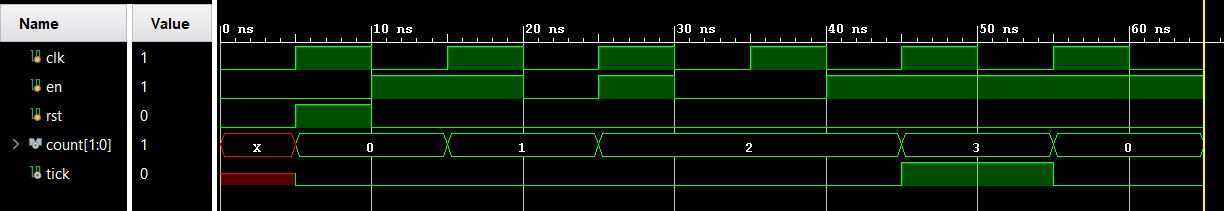
\includegraphics[width=1\textwidth,angle=0,origin=c]{counterWaveform}
	\caption{Counter Simulation Waveform and ERT}
	\label{fig:sim_with_table}
\end{figure}

\begin{figure}[ht]\centering
	
	\begin{tabular}{l|rrrrrrrrrr}
		Time (ms): & 0-2 & 2-4 & 4-6 & 6-8 & 8-10 & 10-12 & 12-14 & 14-16 & 16-18 & 18-20\\
		\midrule
		data  & 41 & 82 & 103      & 204 & 41 & 	  82 & 103 & 	   204 & 41 & 82 \\
		sign  & 0 & 0 & 0      & 0 & 0 &   	  0 & 0 & 	   0 & 1 & 1 \\
		hexDec & 0& 0 & 0      & 0 & 1 &      1 & 1 &      1 & 1 & 1 \\ 
		\midrule
		seg   & 79 & 24$to$0 & 40$to$79 & 79$to$24 & 40 & 40 & 10$to$12 & 79 & 40 & 3f \\
		an    & e  & e$to$d & d$to$b & b$to$7 & 7 & 7$to$e & e$to$d & d$to$b & b & b$to$7 \\
		dp    & 1  & 1      & 1      & 1      & 1 &      1 & 1      & 1      & 1 & 1      \\ 
		\bottomrule
	\end{tabular}
	\bigskip
	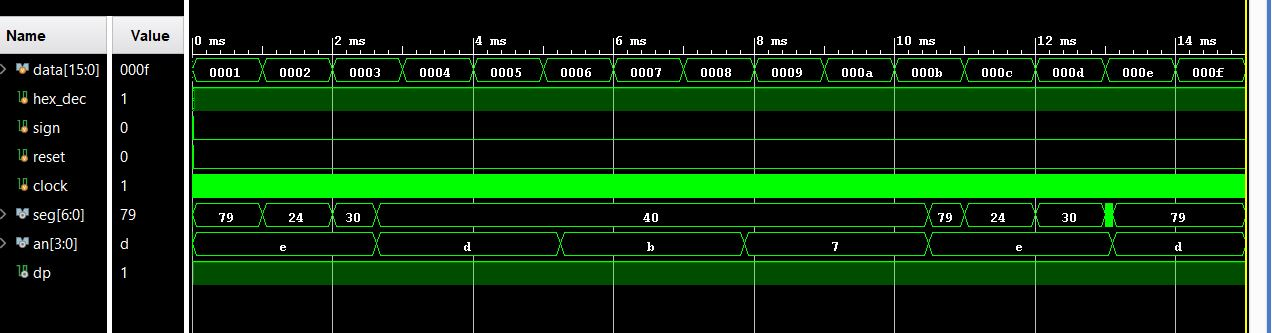
\includegraphics[width=1\textwidth,angle=0,origin=c]{sseg4tdmWaveform}
	\caption{sseg4TDM Simulation Waveform and ERT}
	\label{fig:sim_with_table}
\end{figure}

\begin{figure}[ht]\centering
	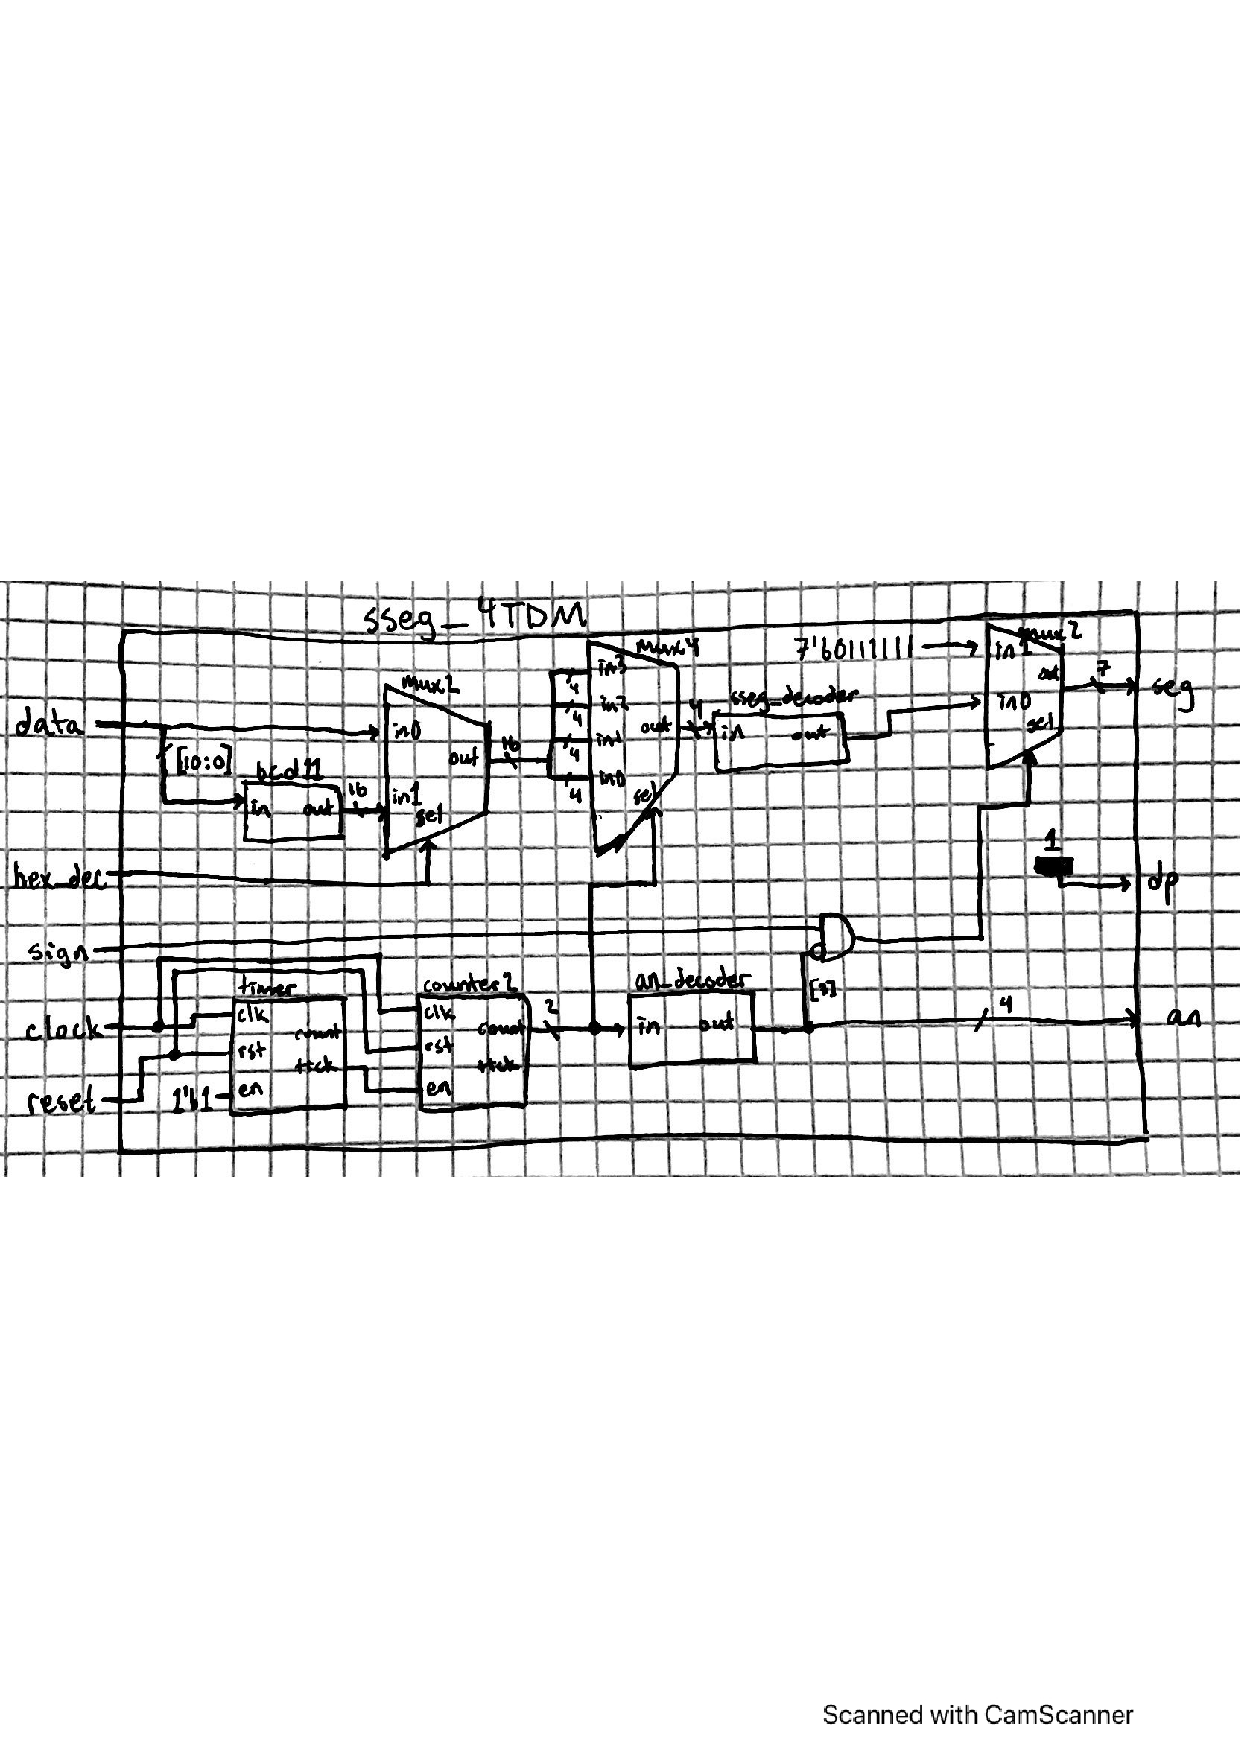
\includegraphics[width=1\textwidth,trim =0 200 0 0,clip, angle=0,origin=c]{sseg4tdmdiagram}
	\caption{sseg4tdm Schematic}
	\label{fig:sim_with_table}
\end{figure}

\begin{figure}[ht]\centering
	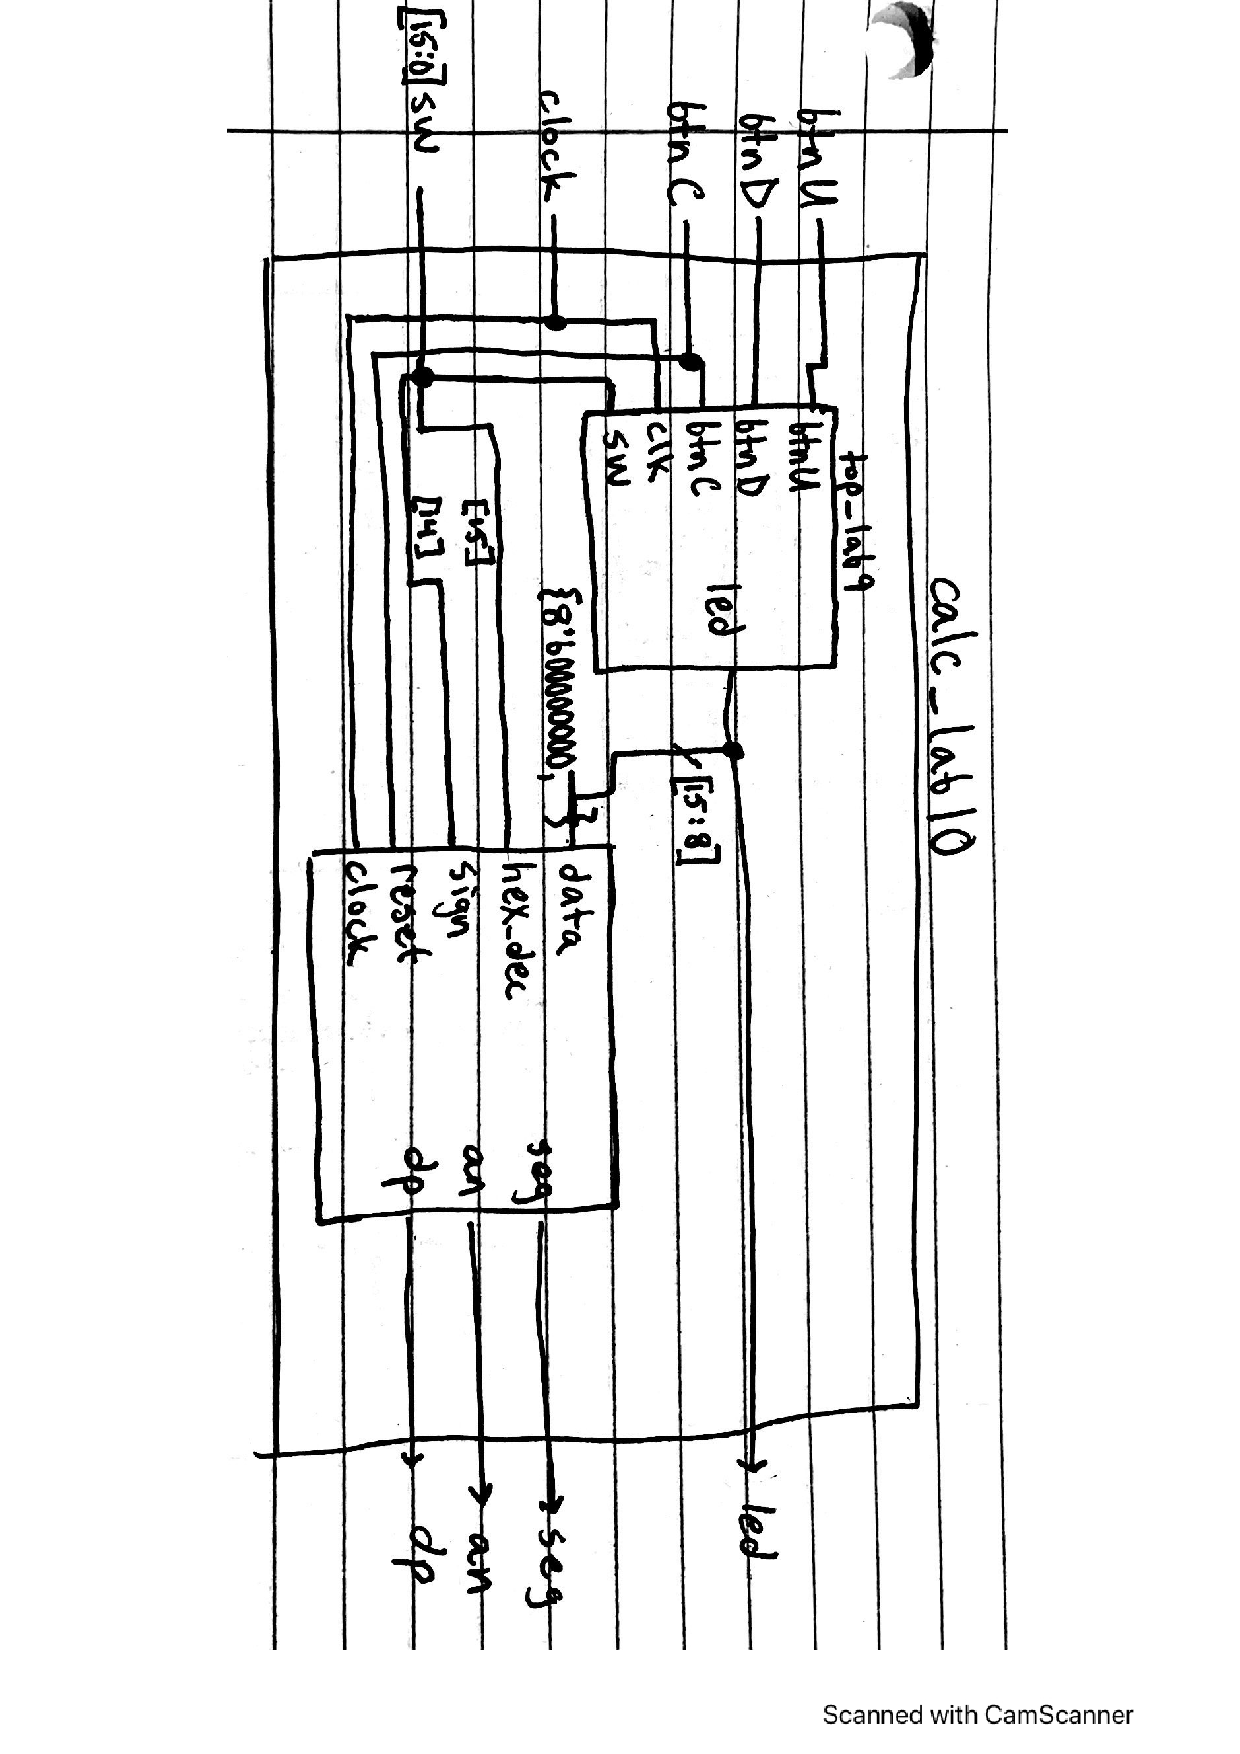
\includegraphics[width=0.65\textwidth,trim =0 0 0 0,clip,angle=90,origin=c]{calclab10diagram}
	\caption{calclab10 Schematic}
	\label{fig:sim_with_table}
\end{figure}

\clearpage
\section*{Code}

\begin{lstlisting}[style=Verilog,
caption=Counter Source Code,
label=MUX w/ two inputs Source Code
]
	module counter #(parameter N=1) 
		( 
		input clk, rst, en,
		output [N-1:0] count, 
		output tick 
		);
		
		// internal signals
		reg [N-1:0] Q_reg , Q_next;
		
		// register (state memory)
		always @(posedge clk, posedge rst) 
		begin
			if (rst) 
				Q_reg <= 0; 
			else
				Q_reg <= Q_next;
		end
		
		// next -state logic 
		always @* 
			begin 
			if (en) 
				Q_next = Q_reg + 1; 
			else 
				Q_next = Q_reg; // no change 
		end
		
		// output logic 
		assign count = Q_reg; 
		assign tick = (Q_reg=={N{1'b1}}) ? 1'b1 : 1'b0;
	
	endmodule
\end{lstlisting}
\clearpage

\begin{lstlisting}[style=Verilog,
caption=Counter Test,
label=MUX2 Test
]
	module counterTest();
	
		reg clk, en, rst;
		wire [1:0] count;
		wire tick;
		
		counter #(.N(2)) c(.count(count), .clk(clk),
			.en(en), .rst(rst),
			.tick(tick) );
	
		always begin 
			clk = ~clk; #5; 
		end
		
		// this block only runs once
		initial begin
			clk=0; en=0; rst=0; ; #5;
			rst = 1; #5;
			// reset
			en = 1; rst = 0; #10;
			en = 0;     #5;
			en = 1;     #5;
			en = 0;     #10;
			en = 1;     #5;
			$finish;
		end 
	endmodule
\end{lstlisting}

\begin{lstlisting}[style=Verilog,
caption= Sseg4TDM Source Code,
label=MUX w/ four inputs Source Code
]
	module sseg4_TDM(
		input [15:0]data,
		input hex_dec, sign,
		input reset, clock,
		output [6:0] seg,
		output [3:0] an,
		output dp
		);
		
		wire [15:0] mux2mux4, bcd2mux2;
		wire [6:0] ssegmux2;
		wire [3:0] mux4sseg, anan;
		wire [1:0] digit_sel;
		wire andmux2;
		wire timer2counter;
		
		bcd11 bcd11in(
			.in(data[10:0]),
			.out(bcd2mux2)
			);
		mux2 #(.N(16)) mux2num1(
			.in0(data), .in1(bcd2mux2), .sel(hex_dec),
			.out(mux2mux4)
			);
		mux4 mux4num1(
			.in3(mux2mux4[15:12]), .in2(mux2mux4[11:8]), 
			.in1(mux2mux4[7:4]), .in0(mux2mux4[3:0]),
			.sel(digit_sel),
			.out(mux4sseg)
			);
		sseg_decoder ssegdecode(
			.in(mux4sseg),
			.out(ssegmux2)
			);
		mux2 #(.N(7)) mux2num2(
			.in1(7'b0111111), .in0(ssegmux2), .sel(andmux2),
			.out(seg[6:0])
			);
		and A1(
			andmux2,
			sign, ~anan[3]
			);
		an_decoder andecode(
			.in(digit_sel),
			.out(anan)
			);
		
		counter #(.N(18)) timer(
			.en(1'b1), .clk(clock), .rst(reset),
			.count(), .tick(timer2counter)
			);
		
		counter #(.N(2)) counter2(
			.en(1'b1), .clk(timer2counter), .rst(reset),
			.count(digit_sel), .tick()
			);
		
		assign an = anan;
		assign dp = 1;
	
	endmodule
\end{lstlisting}
\clearpage
\begin{lstlisting}[style=Verilog,
caption=Sseg4TDM Test,
label=MUX4 Test
]
	module sseg4_TDMTEST();
	
		reg [15:0]data;
		reg hex_dec, sign;
		reg reset, clock;
		wire [6:0] seg;
		wire [3:0] an;
		wire dp;
		
		sseg4_TDM  s(.data(data), .hex_dec(hex_dec),
			.sign(sign), .reset(reset), .clock(clock),
			.seg(seg), .an(an), .dp(dp)
			);
		
		always begin 
			clock = ~clock; #5; 
		end
		
		// this block only runs once
		initial begin
			clock = 0; reset=0; #5;
			reset = 1; #5;
		
			// reset
			reset = 0; sign = 0; hex_dec = 0; 
			data = 16'b0000000001000001; #2000000;
			data = 16'b0000000010000010; #2000000;
			data = 16'b0000000100000011; #2000000;
			data = 16'b0000001000000100; #2000000;
			reset = 0; sign = 0; hex_dec = 1; 
			data = 16'b0000000001000001; #2000000;
			data = 16'b0000000010000010; #2000000;
			data = 16'b0000000100000011; #2000000;
			data = 16'b0000001000000100; #2000000;
			reset = 0; sign = 1; hex_dec = 1; 
			data = 16'b0000000001000001; #2000000;
			data = 16'b0000000010000010; #2000000;
			data = 16'b0000000100000011; #2000000;
			data = 16'b0000001000000100; #2000000;
			
			$finish;
		end 
	endmodule
\end{lstlisting}
\clearpage
\begin{lstlisting}[style=Verilog,
caption=CalcLab10,
label=MUX2 Test
]
	module calc_lab10(
		input btnU, btnD, clk, btnC,
		input [15:0]sw,
		output [6:0] seg,
		output [3:0] an,
		output [15:0] led,
		output dp
		);
	
	
		top_lab9 calc_unit(
			.btnU(btnU), .btnD(btnD), .clk(clk), .btnC(btnC),
			.sw(sw),
			.led(led)
			);
		
		sseg4_TDM disp_unit(
			.data({8'b00000000, led[15:8]}), .hex_dec(sw[15]),
			.sign(sw[14]), .reset(btnC), .clock(clk),
			.seg(seg), .an(an), .dp(dp)
			);
	
	endmodule
\end{lstlisting}


\end{document}